\documentclass[11pt]{article}
\usepackage{amsmath, amssymb}
\usepackage{geometry}
\geometry{margin=1in}
\usepackage{fancyhdr}
\usepackage{lastpage}
\usepackage{parskip} % Better paragraph spacing
\usepackage{titlesec} % Better section formatting
\usepackage{graphicx}
\usepackage{float}
\usepackage[most]{tcolorbox}
\usepackage{lmodern}
\usepackage{caption}
\usepackage{hyperref}
\usepackage{listings}
\usepackage{xcolor}

% Define code styling
\definecolor{codegreen}{rgb}{0,0.6,0}
\definecolor{codegray}{rgb}{0.5,0.5,0.5}
\definecolor{codepurple}{rgb}{0.58,0,0.82}
\definecolor{backcolour}{rgb}{0.95,0.95,0.92}

\lstdefinestyle{mystyle}{
    backgroundcolor=\color{backcolour},
    commentstyle=\color{codegreen},
    keywordstyle=\color{magenta},
    numberstyle=\tiny\color{codegray},
    stringstyle=\color{codepurple},
    basicstyle=\ttfamily\footnotesize,
    breakatwhitespace=false,
    breaklines=true,
    captionpos=b,
    keepspaces=true,
    numbers=left,
    numbersep=5pt,
    showspaces=false,
    showstringspaces=false,
    showtabs=false,
    tabsize=2
}

\lstset{style=mystyle}

% Define commands for reusable content
\newcommand{\coursename}{COM-407 Advanced Networks}
\newcommand{\lecturenum}{09}
\newcommand{\lecturedate}{13/11/2025}
\newcommand{\professor}{Pavlos Nikolopoulos}

\hypersetup{colorlinks=true,linkcolor=blue,urlcolor=blue}

% Configure section spacing
\titlespacing*{\section}{0pt}{2ex plus 1ex minus .2ex}{1.5ex plus .2ex}
\titlespacing*{\subsection}{0pt}{1.5ex plus 1ex minus .2ex}{1ex plus .2ex}
% Header / Footer
\pagestyle{fancy}
\fancyhf{}
\fancyhead[L]{\coursename}
\fancyhead[R]{Lecture \lecturenum}
\fancyfoot[L]{EPFL - Computer Science}
\fancyfoot[C]{Author: Jonathan Dutoit}
\fancyfoot[R]{Page \thepage\ of \pageref{LastPage}}

\begin{document}

\begin{center}
  {\large EPFL - Computer Science} \\[0.5em]
  {\Large \textbf{\coursename}} \\[0.5em]
  {\large Lecture \lecturenum\ --- \lecturedate} \\[0.5em]
  {\large Author: Jonathan Dutoit} \\[0.5em]
  {\large Professor: \professor} \\[0.5em]
\end{center}

\vspace{2cm}

\begin{center}
  {\LARGE \textbf{Routing Algorithms}}
\end{center}

\vspace{1cm}

\section*{Contents}

1. Routing in General \\
2. Link state routing, OSPF Single Area \\
3. Dijkstra's algorithm \\
4. Equal Cost Multipath \\
5. Topology Changes \\
6. Security of OSPF \\
7. OSPF, multiple areas \\
8. Other uses of Link State \\
9. Software Defined Networking (SDN)

\section*{Reminder: the network layers}

A router has 2 functions:

\textbf{\textcolor{blue}{Forwarding}}: When a packet arrives at a router's input link, the routers moves the packet to the appropriate outgoing link. This is based on: 
\begin{itemize}
	\item Information in the packet header (e.g., dest IP address, BIER extension header, etc.)
	\item the router's \textcolor{purple}{\textit{forwarding table}} (a.k.a \textcolor{purple}{\textit{routing table}})
\end{itemize}

\textcolor{blue}{\textbf{Routing}}: Determines the entire \textcolor{purple}{route/path} followed by each packet towards its destination hence the entries of the forwarding tables and/or information in extension header. This is typically done by a \textit{\textcolor{purple}{routing algorithm}}

\section*{Routing protocols (or routing algorithms)}

\textcolor{red}{\textit{Why we need them?}}
\begin{itemize}
	\item Manually configuring the forwarding tables is \textcolor{red}{not} easy. In a single domain, it's doable but time-consuming and error-prone. In the WAN. it is impossible - about 120000 domains should coordinate. 
	\item A routing protocol or algorithm thus allows routers to \textcolor{blue}{automatically} compute the \textcolor{blue}{best path(s)} to each destination.
\end{itemize}

\textcolor{red}{How they differ?}

\textbf{\textit{Optimization objective of the algorithm}}
\begin{itemize}
	\item To use least-cost path
	\item To use equal-cost multi-path
	\item To respect policies
	\item Arbitrary (min delay, low bandwidth usage...)
\end{itemize}

\textbf{\textit{The underlying network, topology available?}}
\begin{itemize}
	\item Single domain $\Rightarrow$ \textcolor{blue}{infra-domain} routing (main alg. is OSPF)
	\item Multiple domains $\Rightarrow$ \textcolor{blue}{inter-domain} routing (main alg. is BGP)
\end{itemize}

\textbf{\textit{Where is the output stored?}}
\begin{itemize}
	\item Inside a local forwarding table
	\item Directly into the packet headers
\end{itemize}

\section*{Taxonomy of routing protocols}

\textcolor{red}{\textit{Link State}}: Each router maintains a local \textcolor{blue}{\textit{map}} of the entire topology
\begin{itemize}
	\item Obtained by \textit{gossiping} with other routers (flooding)
	\item Every link on map has a cost; e.g. cost (1 Gb/s link) = 1
\end{itemize}
Furthermore, it computes the \textcolor{blue}{shortest (min-cost) paths} to each destination prefix based on map and determines next hop to each prefix and populates its forwarding table. 

It's mainly used for \textit{\textcolor{blue}{intra-domain routing}} (e.g., OSPF, IS-IS) and advanced bridging methods (e.g., TRILL, SPB Shortest Path Bridging)


\textcolor{red}{\textit{Distance Vector}}: \textcolor{blue}{\textit{No}} global map. Each router initially knows only about:
\begin{itemize}
	\item Locally-attached networks and neighbour routers,
	\item And the \textcolor{blue}{costs} of direct links to them
\end{itemize}
Then, it \textbf{\textit{informs}} neighbors about the estimated distances to all destinations it knows (= sends its \textcolor{purple}{distance vector}); \textbf{\textit{learns}} new destinations from vectors received by neighbors and \textbf{\textit{updates}} its distance vector (using the \textcolor{purple}{Bellman-Ford algorithm}).

Finally: it determines next hops and populates its forwarding table.

\begin{minipage}{0.3\textwidth}
\begin{itemize}
	\item All link costs = 1 \\
	\item This message-passing method \textcolor{blue}{\textit{converges}} to shortest paths! \\
	\item But, it may need \textcolor{red}{\textit{time to converge}} \\
	\item Hence it is used in \textcolor{red}{\textit{small}} networks \\
\end{itemize}

\end{minipage}
\hfill
\begin{minipage}{0.7\textwidth}
\centering
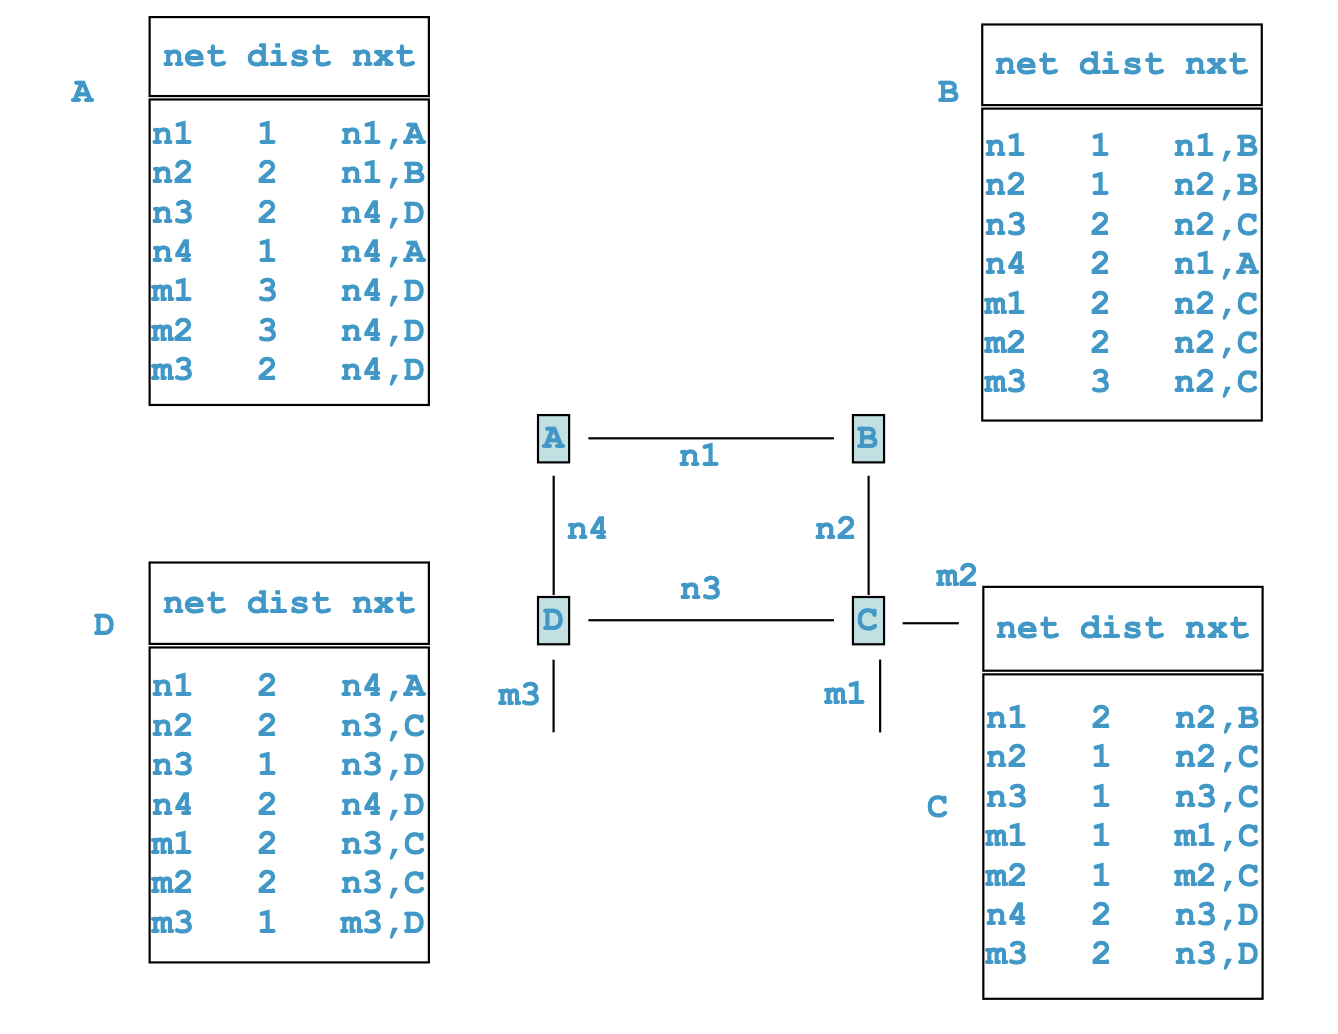
\includegraphics[width=\linewidth]{distance-vector}
\end{minipage}


\textcolor{red}{\textit{Path Vector}}: We don't know the topology nor the costs. Hence, every router knows only:
\begin{itemize}
	\item Its neighbors plus explicit \textcolor{blue}{\textit{paths}} to all destinations 
\end{itemize}
It then computes the "best" path to each destination and populates forwarding table. Optimization criterion is \textcolor{blue}{\textit{not cost}}. 

This is suitable for \textcolor{blue}{\textit{inter-domain routing}}, because it is hard to assign costs and domains may do not want to disclose their private internal topology. Computation may be based on the amount of hops for example. 
\begin{itemize}
	\item e.g., BGP computes domain-level paths
	\item Each router selects best path according to \textit{multiple criteria}
\end{itemize}

\newpage

% Quick centered image
\begin{figure}[H]
    \centering
    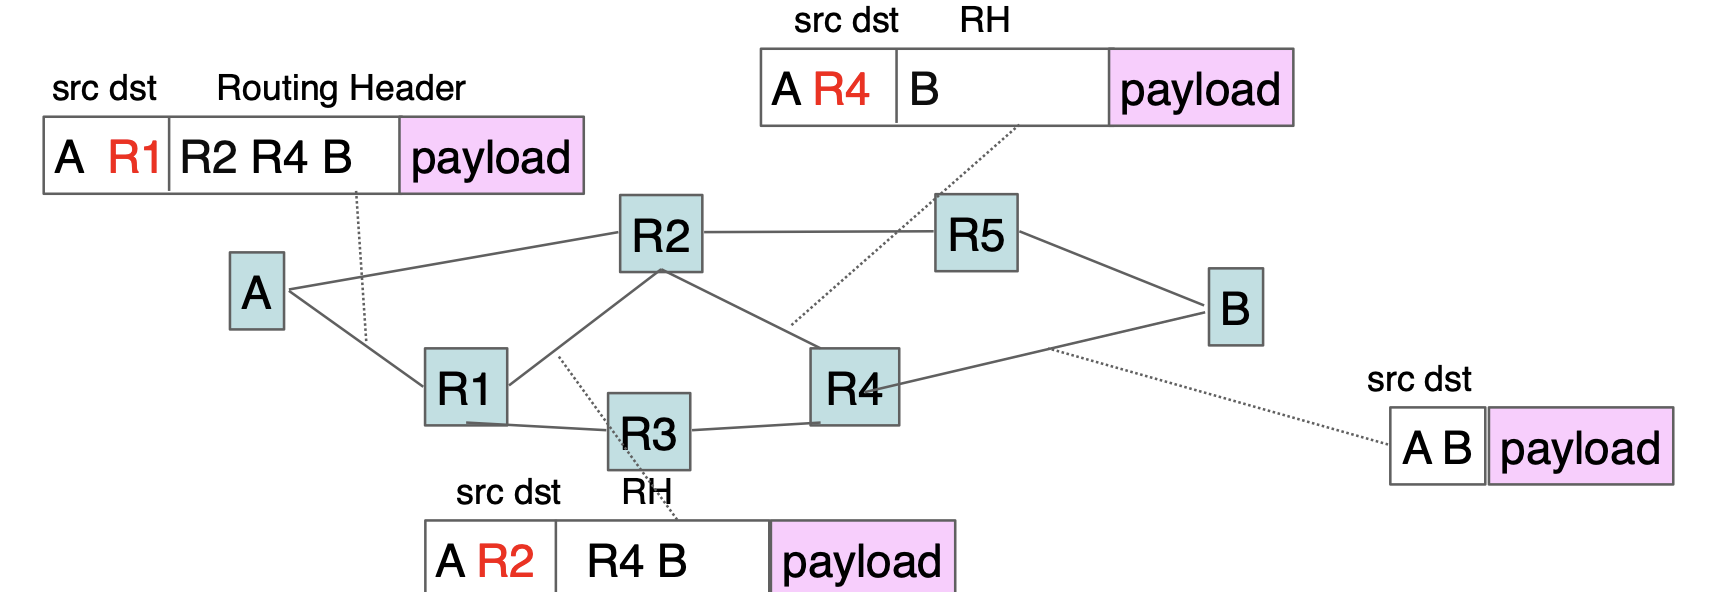
\includegraphics[width=0.8\textwidth]{source-routing-strict}
    \label{fig:LABEL}
\end{figure}

\textcolor{red}{\textit{Source Routing "Strict"}}

\begin{itemize}
	\item Source puts explicit paths \textcolor{blue}{\textit{into packet headers}} (path = sequence of intermediate hops)
	\item In IPv6, routing header is an extension header - contains intermediate hops and ultimate destination; destination IP address is next intermediate hop
	\item Intermediate routers are "dumb": just remove themselves from header and forward packets to next hop
	\item Used in \textcolor{blue}{\textit{ad-hoc networks}}, where route computation is done by a control application or by discovery: e.g.: source discovers path by flooding \textit{explorer packets} that accumulate the path followed
\end{itemize}

% Quick centered image
\begin{figure}[H]
    \centering
    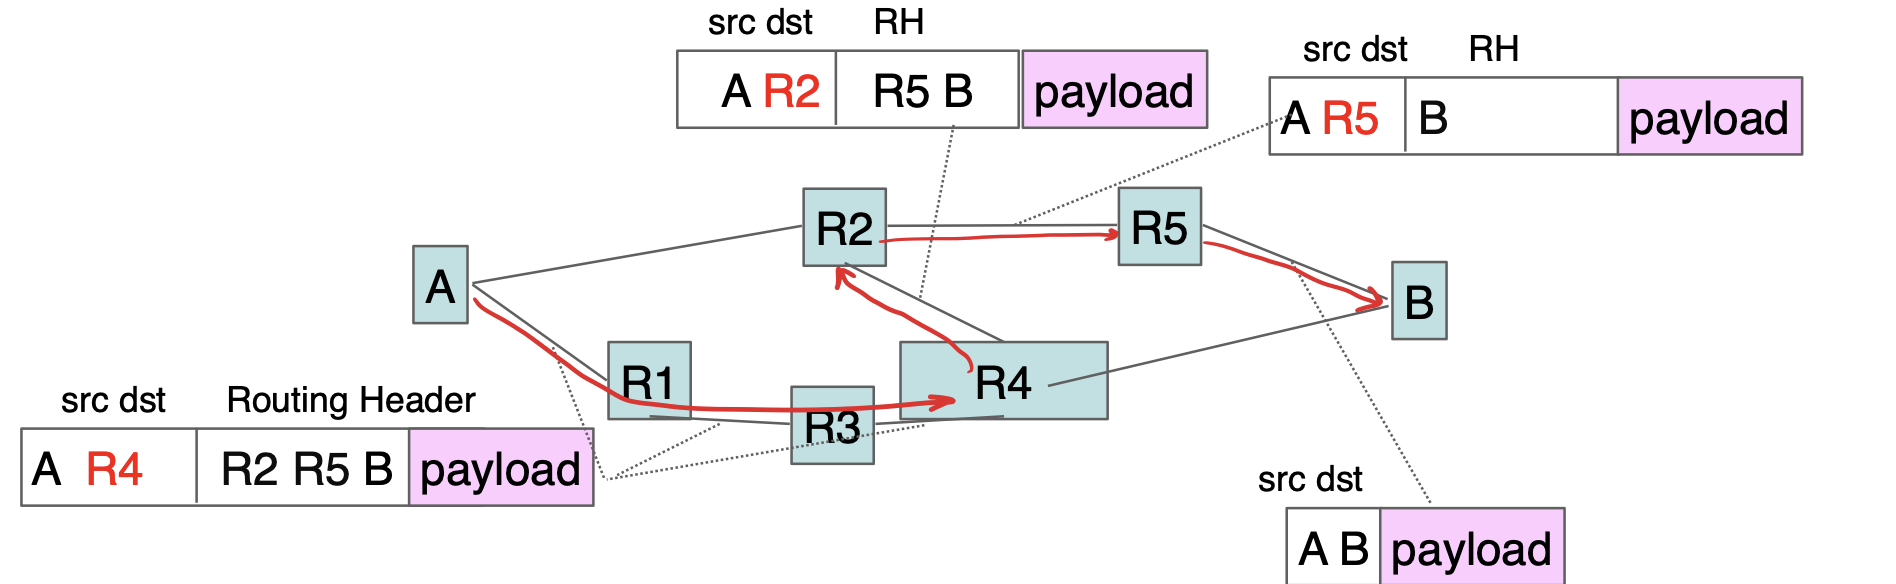
\includegraphics[width=0.8\textwidth]{source-routing-loose}
    \label{fig:LABEL}
\end{figure}

\textcolor{red}{\textit{Source Routing "Loose"}}
\begin{itemize}
	\item Forces \textcolor{blue}{\textit{some}} intermediate hops
	\item Assumes an \textcolor{purple}{\textit{underlying}} routing algorithm such as link-state routing, e.g., we know how to go from A to R4
	\item Used for fine grained control (traffic engineering, separation of costumers)
\end{itemize}

\textcolor{red}{\textit{Segment Routing}}
\begin{itemize}
	\item Generalizes loose source routing by allowing the routing header to contain processing instructions for the intermediate hop: e.g., we can ask R4 to apply a security \textcolor{blue}{\textit{function}} (screening, traffic separation)
	\item Used in data centers
\end{itemize}

\newpage

\section*{2. OSPF (for a single area)}

Most important link state algorithm (\textit{"Each router maintains a local map of the entire topology"}). Every router has:
\begin{itemize}
	\item an \textcolor{blue}{\textit{interface database}} (= its network interfaces, learnt by configuration)
	\item an \textcolor{blue}{\textit{adjacency database}} (= neighbors' states, learnt by a \textcolor{red}{hello} protocol)
	\item a \textcolor{blue}{\textit{link state database}} (= topology map, learnt by flooding)
\end{itemize}

\textcolor{red}{Hello} is a \textbf{\textit{ping-style}} protocol between immediate neighbors
\begin{itemize}
	\item discovers neighbor routers
	\item detects failures (if neighbor doesn't respond after 3 times, it is considered "dead")
\end{itemize}

\subsection*{Link State Database and LSAs}

When two routers become neighbors, they first \textcolor{red}{\textit{synchronize}} their link state databases:
\begin{itemize}
	\item \textbf{Case 1}: one router is new, hence \textcolor{blue}{\textit{copies}} what the other already knows
	\item \textbf{Case 2:} existing routers connect, hence they \textcolor{blue}{\textit{merge}} their database
\end{itemize}

Once synchronized, a router sends and accepts \textcolor{red}{\textit{link state advertisements (LSAs):}}
\begin{itemize}
	\item Every router sends a LSA with its attached networks and neighbor routers
	\item LSAs are \textcolor{red}{\textit{flooded}} in the entire area and stored in each router's link state database
	\item LSAs contains a \textcolor{blue}{\textit{sequence}} number and \textcolor{blue}{\textit{age}}. Sequence number prevents loops since only messages with new sequence numbers are accepted and re-flooded; Age field is used to periodically resend LSA and to flush invalid LSAs
\end{itemize}

\subsection*{Example showing interface databases}

% Quick centered image
\begin{figure}[H]
    \centering
    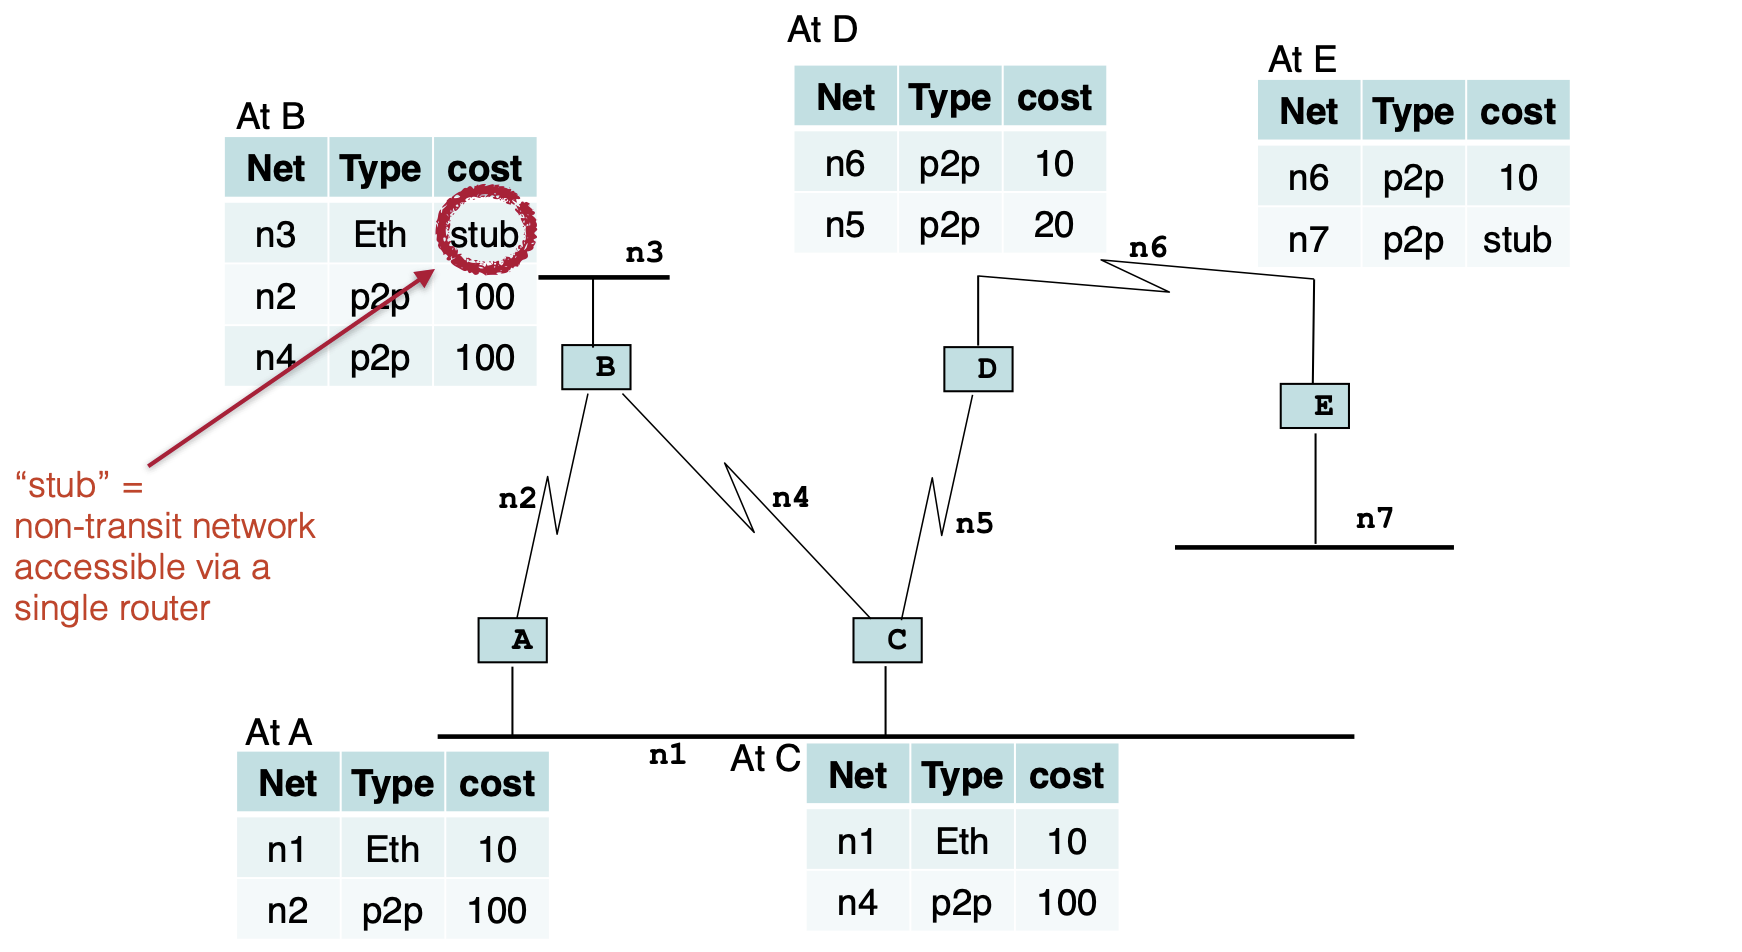
\includegraphics[width=0.9\textwidth]{interface-databases}
    \label{fig:LABEL}
\end{figure}

\section*{Routers flood their LSAs throughout area}

% Quick centered image
\begin{figure}[H]
    \centering
    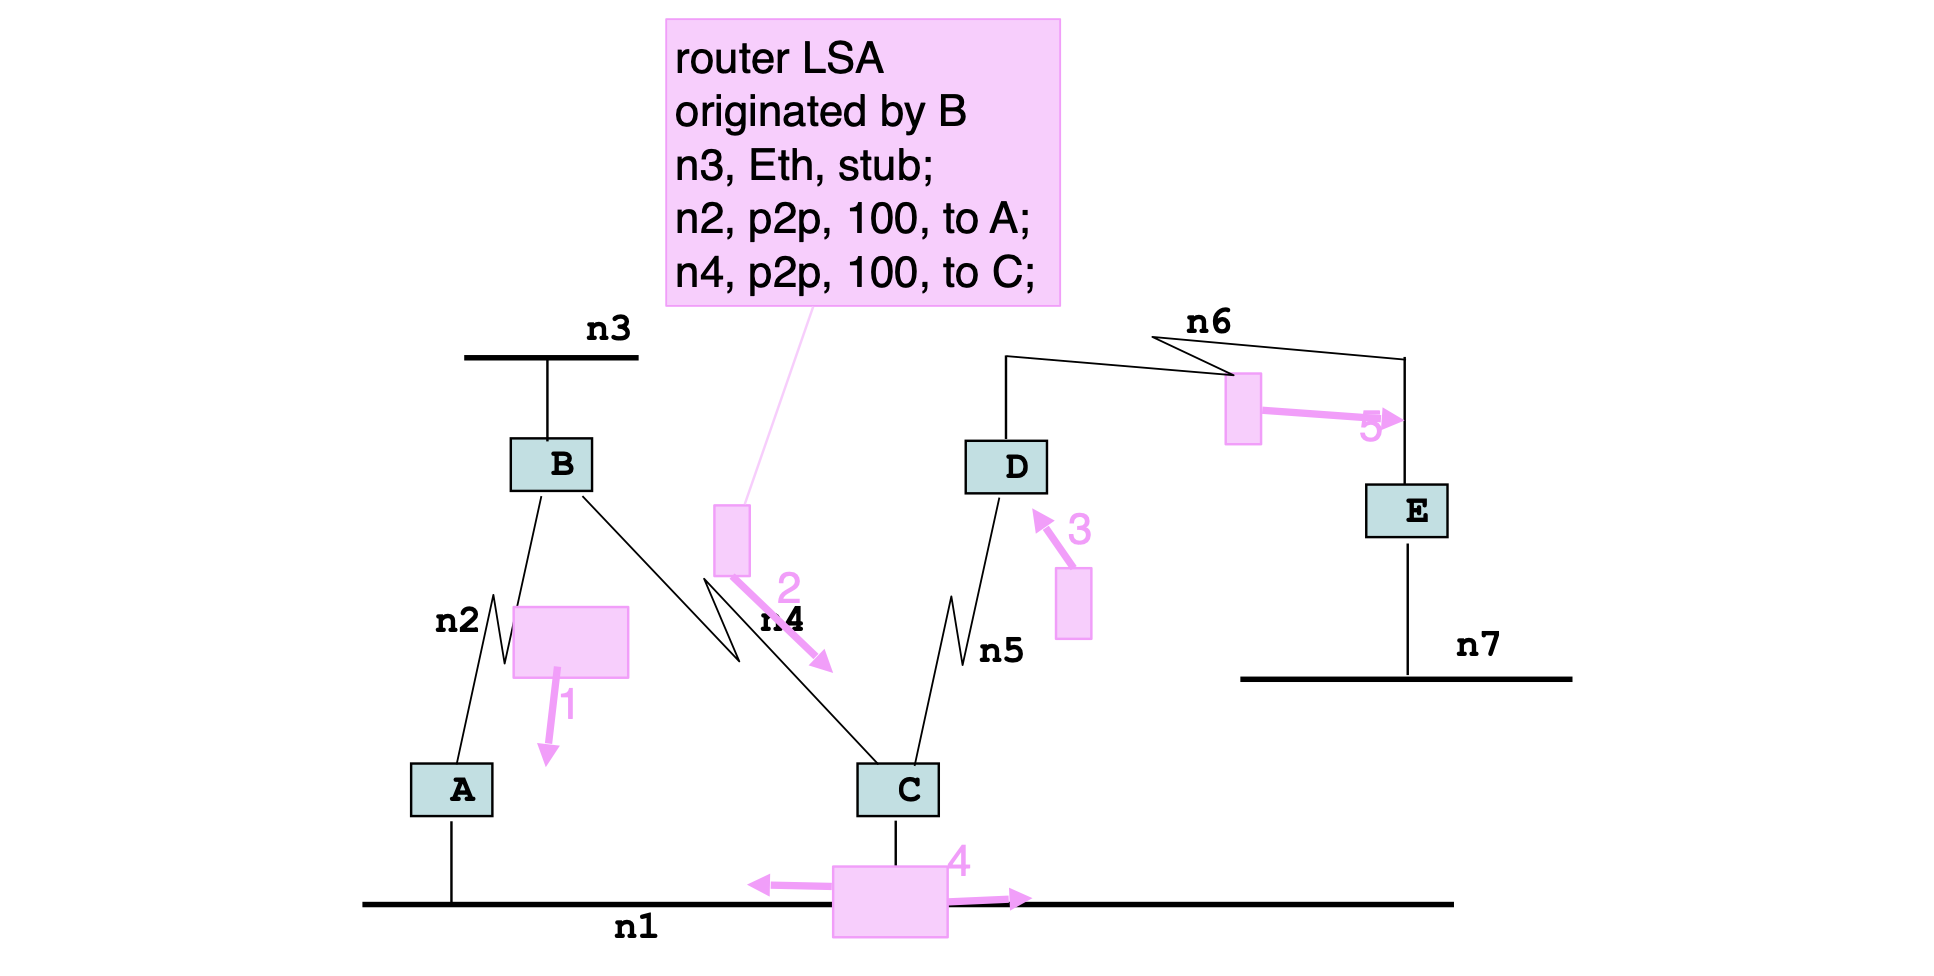
\includegraphics[width=1\textwidth]{routers-flood}
    \label{fig:LABEL}
\end{figure}

\begin{itemize}
	\item The LSA describes all the networks attached to B and their costs, as well as the adjacent routers
	\item A "stub" network means non transit, i.e. there is no other router on this network. A stub network can be reached by only a single router; so, all we need to know is how to reach this router. No need to allocate a cost to a stub network. 
\end{itemize}

\subsection*{After flooding}
% Quick centered image
\begin{figure}[H]
    \centering
    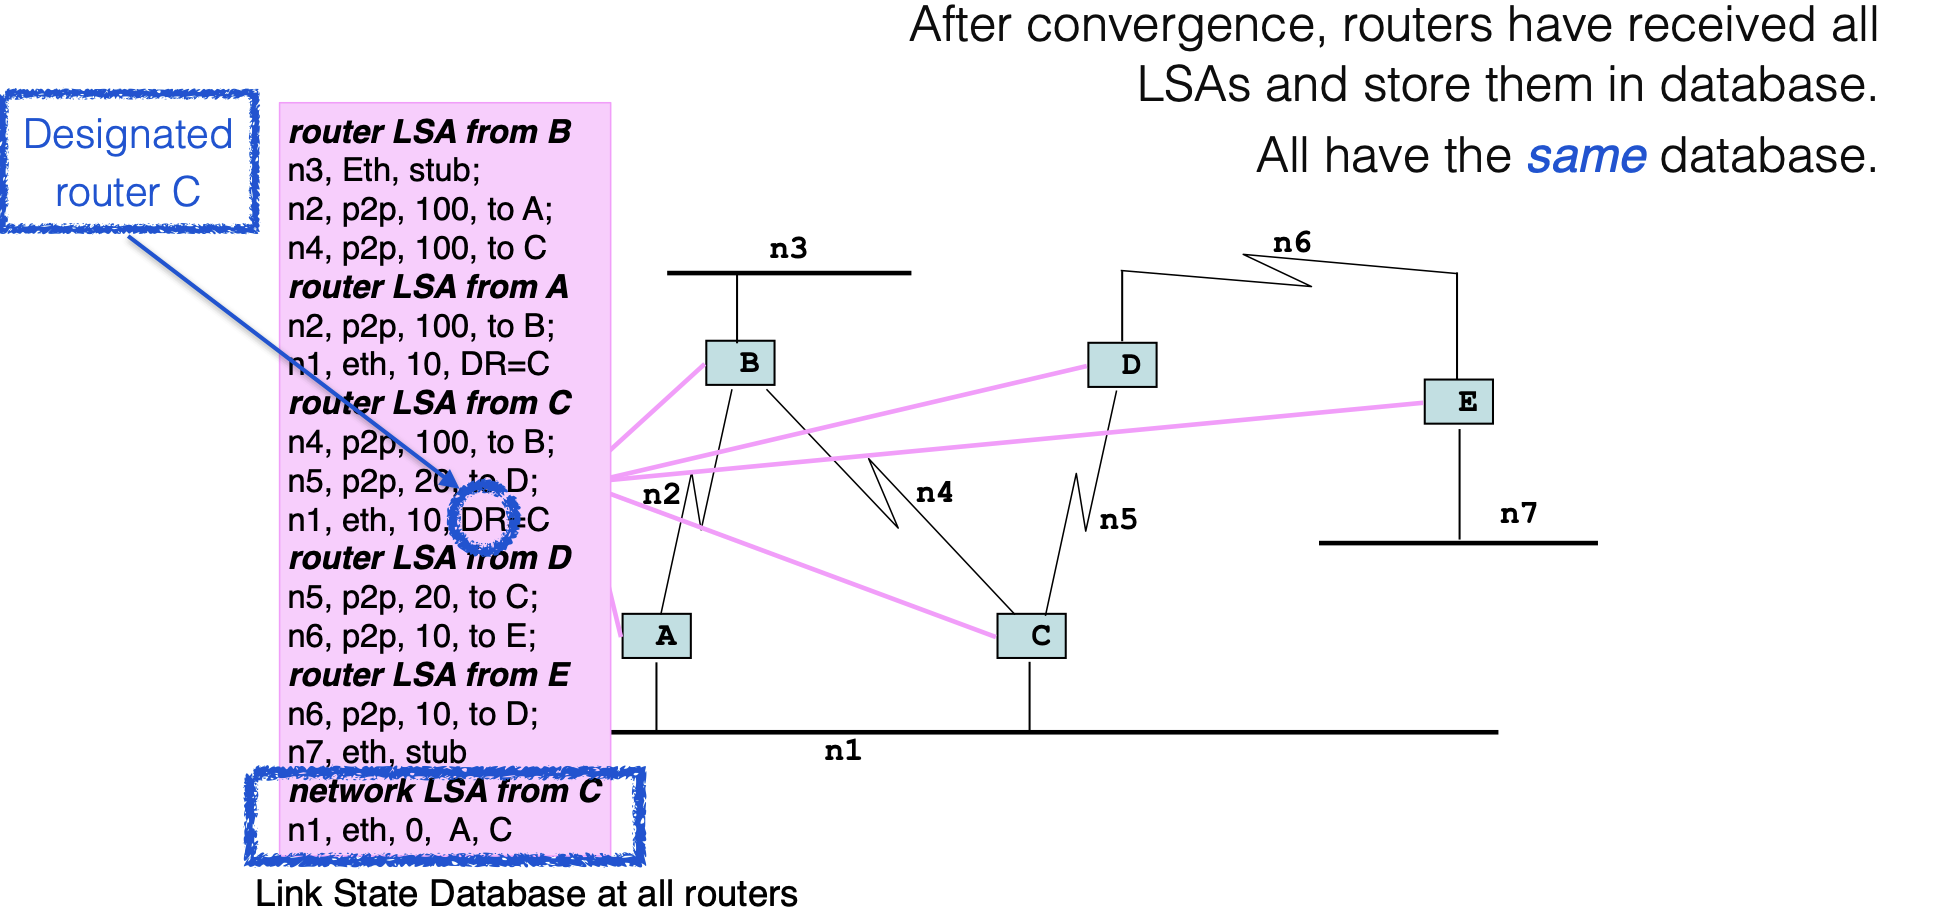
\includegraphics[width=1\textwidth]{after-flooding}
    \label{fig:LABEL}
\end{figure}

\begin{itemize}
	\item In order to avoid issues as high number of OSPF packets that are sent and processed by each router as well as redundancy in case of failures, the routers elect a \textcolor{red}{designated router} per LAN (and a backup designated router)
	\item The designated router is typically the oldest running router and "speaks for the switch" and sends a "\textcolor{red}{network LSA}" which gives the list of all routers connected to the LAN.
\end{itemize}

\subsection*{New Router Boots}

% Quick centered image
\begin{figure}[H]
    \centering
    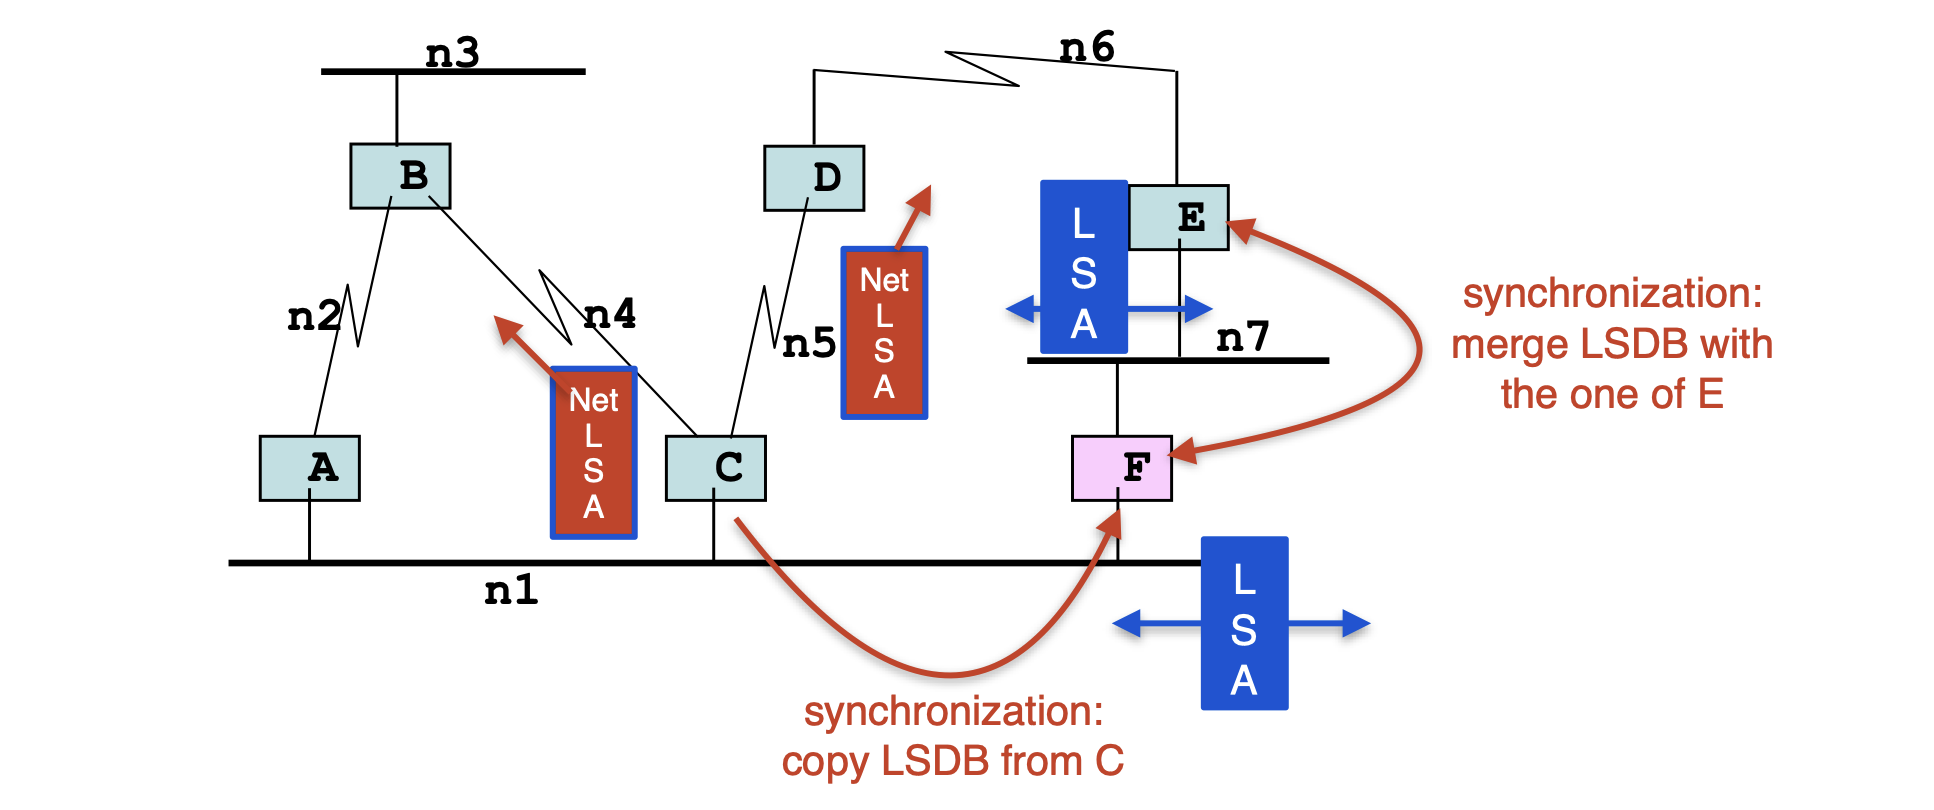
\includegraphics[width=1\textwidth]{new-router}
    \label{fig:LABEL}
\end{figure}

\begin{itemize}
	\item Synchronization steps: boot up, identify neighbors, check designated router and copy their database
	\item After that, F starting issues new LSAs. C will also issue new LSAs saying "F is new member of this network"
	\item Finally, establish adjacency with other network, and you do the same thing with E (merging own views of topologies). E will send its new version of the LSAs 
\end{itemize}

\subsection*{From LSDB to Topology Graph}

% Quick centered image
\begin{figure}[H]
    \centering
    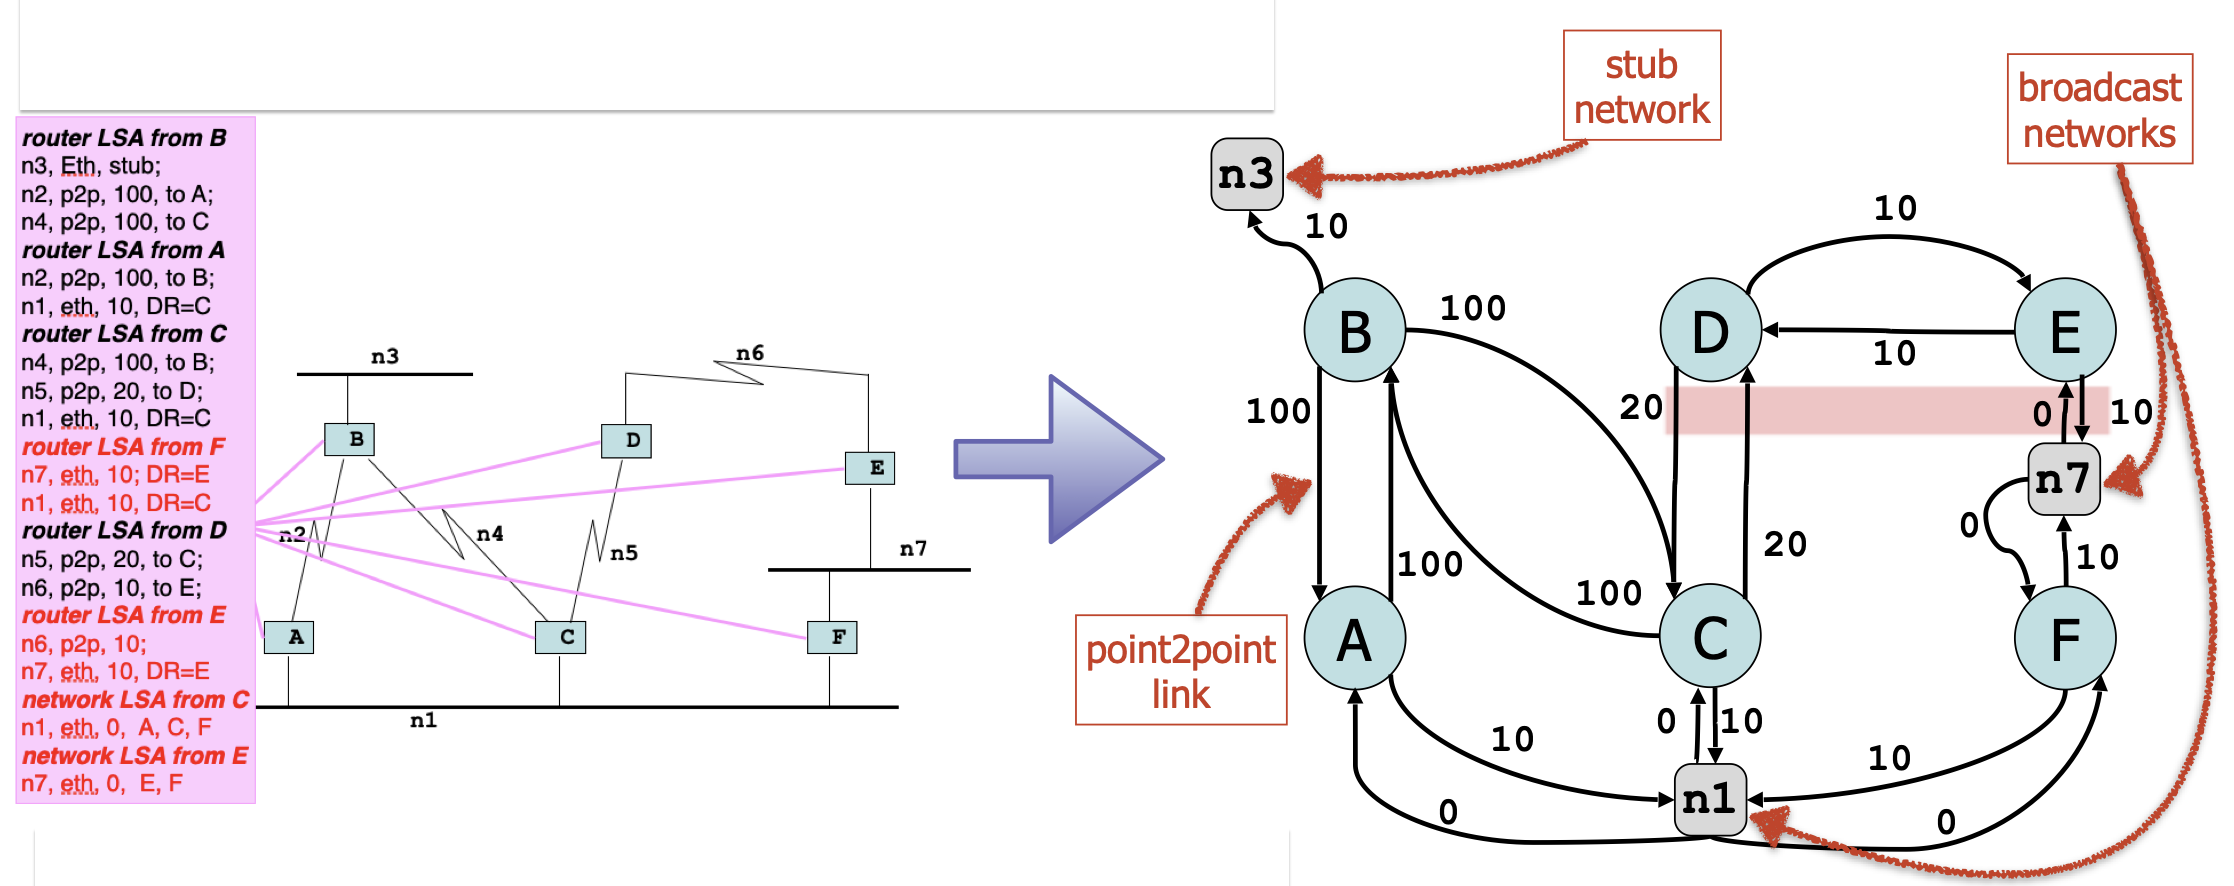
\includegraphics[width=1\textwidth]{topology-graph}
    \label{fig:LABEL}
\end{figure}

\subsection*{Practical Aspects}
\begin{itemize}
	\item OSPF packets are sent \textcolor{blue}{\textit{directly over IP}} 
	\item Reliable transmission is managed by OSPF using \textbf{acknowledgements} and \textbf{timers} (like the \textcolor{blue}{\textit{stop and go}} protocol)
	\item Routers IDs or Area IDs are 32 bit numbers
\end{itemize}

\section*{3. Shortest paths are found with Dijkstra's Algorithm}

Each router runs Dijkstra \textcolor{red}{\textit{independently}} on its local LSDB copy. \textit{Why?}
\begin{itemize}
	\item every router computes \textcolor{blue}{\textit{shortest paths starting from itself}}
	\item LSAs guarantee \textcolor{blue}{\textit{no persistent}} inconsistencies (LSDBs are mostly identicaly)
\end{itemize}

Also, each router computes \textcolor{red}{\textit{one or several}} shortest paths to every other node

\subsection*{Dijkstra's Shortest Path Algorithm}
\texttt{
m(0) = 0; m(i) = $\infty$ $\forall$ $i$ $\neq$ 0; $V = \emptyset$; pred(i) = $\emptyset$ $ \forall i$;
}
\begin{lstlisting}[language=Octave]
for k = 0:N do
	find i not in V that minimizes m(i)
	if m(i) is finite
		add i to V
		for all neighbors j not in V of i
			if m(i) + c(i, j) < m(j)
				m(j) = m(i) + c(i, j)
				pred(j) = [i]
			else if m(i) + c(i, j) = m(j)
				m(j) = m(i) + c(i, j)
				pred(j) = pred(j) U [i]
\end{lstlisting}

This pseudo-code builds the shortest path tree from this node to all other nodes. 

The line \texttt{find i not in V that minimizes m(i)} adds \textcolor{blue}{\textit{one node at a time}} to the set \textbf{\textit{V}} of visited nodes, by picking the node that is \textbf{\textit{closest}} to the source in terms of least cost path}

\textbf{Note:} There are multiple version of Dijkstra's algorithm. The version presented above finds all shortest paths, other version find only one shortest path to every destination. The version presented is very close to what is really implemented in OSPF (with a difference, next-hop versus pred())

The worst-case complexity of this version is \textbf{\textit{O($N^{2}$)}} where \textit{N} is the number of nodes. More efficient versions of the algorithm have a smaller complexity \textit{O(NlogN + E)} where \textit{E} is the number of links.

\subsection*{Path Computation}
\begin{itemize}
	\item \verb|pred(i)| is the set of predecessors of node \textit{i} on all shortest paths from source to \textit{i}
	\item Shortest paths can be computed \textcolor{red}{\textit{backwards}}, using pred(), starting \textcolor{red}{\textit{from destination}}
\end{itemize}

\subsection*{From shortest paths to Forwarding Table}

Router A keeps in its forwarding table only the \textcolor{blue}{\textit{next-hop}} ad the \textcolor{blue}{\textit{distance}} to every destination (\textcolor{red}{not the entire path}):

% Quick centered image
\begin{figure}[H]
    \centering
    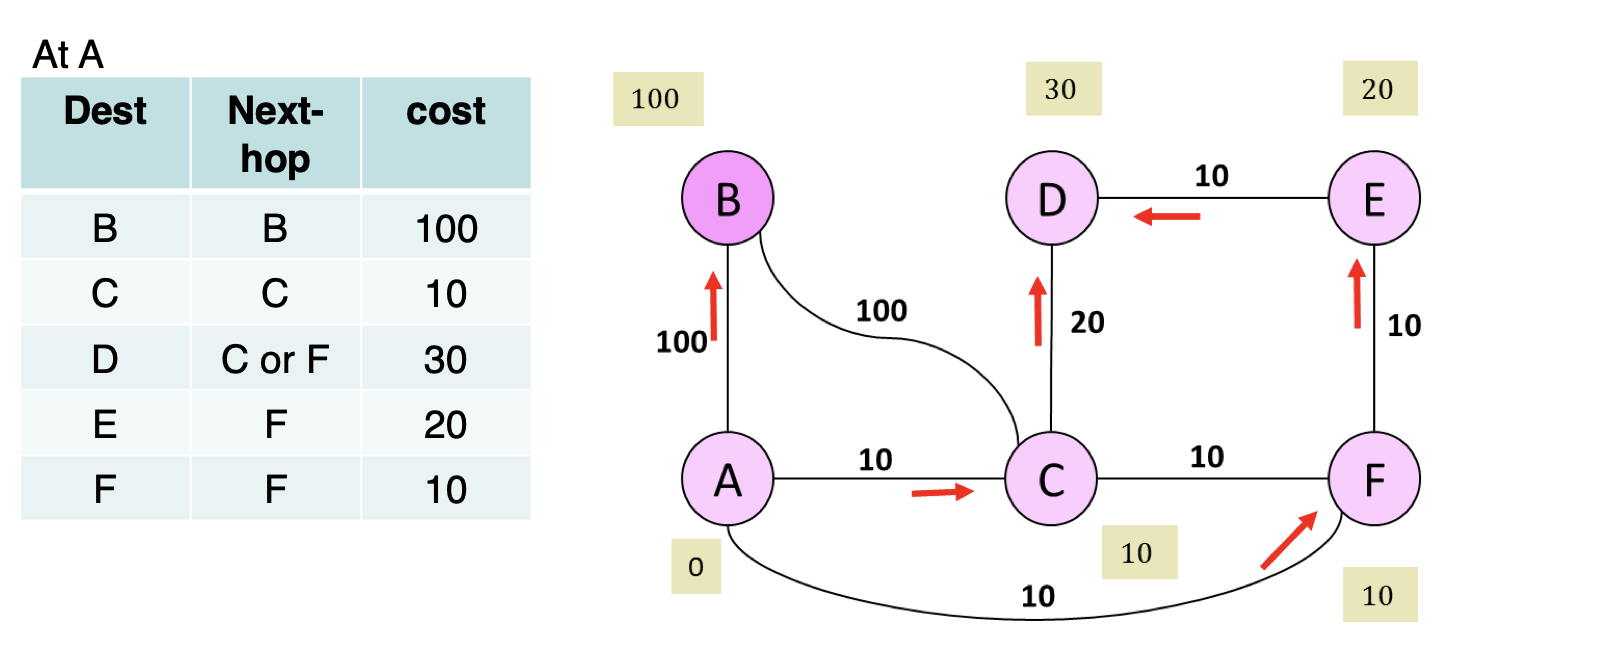
\includegraphics[width=0.8\textwidth]{shortest-paths}
    \label{fig:LABEL}
\end{figure}

\subsection*{Bringing back the Network Nodes}

In practice OSPF adds to the graph the network nodes, which makes the graph \textbf{\textit{larger}}

To optimize computation:
\begin{itemize}
	\item First, stub networks \textcolor{red}{\textit{are removed}}
	\item Then, Dijkstra is run and the forwarding table contains costs and next hop to edge routers
	\item Finally, stub networks are \textcolor{blue}{\textit{added to the forwarding table}} one by one, using information about edge routers.
\end{itemize}

\section*{4. Equal Cost Multipath}

OSPF supports multiple shortest paths. IP allows to have multiple next-hops to the same destination in the forwarding table
\begin{itemize}
	\item good: it exploits the \textcolor{blue}{\textit{redundancy}} of paths
	\item bad: the number of multiple paths may be \textcolor{red}{\textit{large}} so, typically, we use a \textbf{\textit{limit}} of multiple paths
\end{itemize}

\begin{tcolorbox}[
  colback=gray!15,     % background color
  colframe=black!50,    % border color
  boxrule=1pt,       % border thickness
  arc=3mm,             % rounded corners
  left=4mm, right=4mm, top=2mm, bottom=2mm % padding
]
\textbf{What should router A do when it has several packets to send to destination D?}

A. Send them to next-hop F or C randomly with equal probability \\
B. Choose one next-hop and send all packets to this next-hop \\
C. Test the availability of the next-hop before sending \\
D. Something else \\
E. I don't know \\

\textbf{Answer:} A and D. It's better to use \textbf{all} available paths network (\textcolor{blue}{load balancing}) $\Rightarrow$ send to all next-hops with equal probability. \\

However, this may cause \textcolor{red}{\textit{packet re-ordering}} $\Rightarrow$ alternative approach: \textcolor{blue}{\textit{per-flow load balancing}} requires that packets of the same flow to be sent to the same next-hop. 

\vspace{0.3cm}

Text
\end{tcolorbox}
\end{document}
